\documentclass[aspectratio=169]{beamer}

\setlength{\headheight}{26pt}

% Packages
\usepackage[left=25mm, right=25mm, top=35mm, bottom=25mm]{geometry} % defines whitespaces on the edges
\usepackage[bottom, hang]{footmisc}
\usepackage{hyperref}             % for \nameref and cite
\usepackage{footnotebackref}      % used for getting back from the footnote to the main text
\usepackage{enumitem}
\usepackage{graphicx}
\usepackage{fancyhdr}
\usepackage{lastpage}
\usepackage[export]{adjustbox}
\usepackage{float}
\usepackage[ngerman]{babel}
\usepackage[ngerman]{datetime}
\usepackage{apacite}
\usepackage[utf8]{inputenc}
\usepackage{listings}
\usepackage{xcolor}
\usepackage{pdfpages}
\usepackage{url}
\usepackage{outlines}
\usepackage{tocloft}
\usepackage[utf8]{inputenc}
\usepackage{amsmath}
\usepackage{mathtools}
\usepackage[acronym]{glossaries}
\usepackage{titlesec}             % for \titleformat
\usepackage{textcomp}             % for \degree sign
\usepackage{gensymb}              % for \degree sign
\usepackage{csvsimple}            % for using csv-files for tables
\usepackage{lscape}               % for landscape mode
\usepackage{parskip}              % inserts space after paragraph automatically
\usepackage{svg}                  % used to include svg with the help of inkscape which converts svg to pdf
\usepackage{wasysym}              % for \diameter symbol
\usepackage{xfrac}                % for \sfrac

\frenchspacing  % Use same space size between words and between sentences

% change section titles' font size
\titleformat*{\section}{\huge\bfseries}
\titleformat*{\subsection}{\LARGE\bfseries}
\titleformat*{\subsubsection}{\Large\bfseries}
\titleformat{\paragraph}[hang]{\large\bfseries}{\theparagraph}{1em}{}
\titleformat{\subparagraph}[hang]{\normalsize\bfseries}{\thesubparagraph}{1em}{}

\definecolor{codegreen}{rgb}{0,0.6,0}
\definecolor{codegray}{rgb}{0.5,0.5,0.5}
\definecolor{codepurple}{rgb}{0.58,0,0.82}
\definecolor{codeorange}{rgb}{1,0.5,0.15}
\definecolor{backcolour}{rgb}{0.9,0.9,0.9}

\lstdefinestyle{mystyle}{
    backgroundcolor=\color{backcolour},
    commentstyle=\color{codegreen},
    keywordstyle=\color{magenta},
    numberstyle=\tiny\color{codegray},
    stringstyle=\color{codepurple},
    basicstyle=\ttfamily\footnotesize,
    breakatwhitespace=false,
    breaklines=true,
    captionpos=b,
    keepspaces=true,
    numbers=left,
    numbersep=5pt,
    showspaces=false,
    showstringspaces=false,
    showtabs=false,
    tabsize=4
}
\lstset{style=mystyle}

\lstset{
    literate={~} {$\sim$}{1}
}

\lstset{%
    breaklines=true,
    breakatwhitespace=true,
}

\DeclarePairedDelimiter\abs{\lvert}{\rvert} % make scalable absolute stripes
\DeclarePairedDelimiter\parenth{(}{)} % make scalable parentheses

\let\phi\varphi{} % change style of \phi sign

\setlength{\parindent}{0mm} % disable paragraph indent

\newdateformat{mydate}{\THEDAY{. }\monthnamengerman[\THEMONTH] \THEYEAR}

\renewcommand{\listfigurename}{}
\renewcommand\contentsname{Inhaltsverzeichnis}
\renewcommand\lstlistingname{Code}

\makeglossaries{}

% Header/Footer Setting
\setlength\footnotemargin{15pt}
\pagestyle{fancy}
\fancyhf{}
\renewcommand{\footrulewidth}{0.4pt} % footer line
\rhead{\textbf{\vUniversity}\\\vModule}
\lhead{\textbf{\vTitle}\\
    Projektarbeit}
\lfoot{\vAuthorFirstName{} \vAuthorLastName}
\cfoot{\mydate\today}
\rfoot{S.~\thepage~/~\pageref{LastPage}}

% Redefine the plain page style, otherwise there is no header and footer for chapter pages
\fancypagestyle{plain}{%
    \fancyhf{}
    \renewcommand{\footrulewidth}{0.4pt} % footer line
    \rhead{\textbf{\vUniversity}\\\vModule}
    \lhead{\textbf{\vTitle}\\
        Projektarbeit}
    \lfoot{\vAuthorFirstName{} \vAuthorLastName}
    \cfoot{\mydate\today}
    \rfoot{S.~\thepage~/~\pageref{LastPage}}
}

\bibliographystyle{apacite}

% Settings for the equation list
\newcommand{\listequationsname}{}
\newlistof{myequations}{equ}{\listequationsname}
\renewcommand{\cftmyequationsaftersnum}{\hfill}
\renewcommand{\cftmyequationspresnum}{\hfill}
\setlength{\cftmyequationsnumwidth}{3.5em}
\newcommand{\myequations}[1]{%
\addcontentsline{equ}{myequations}{\protect\numberline{\theequation}#1}\par}

\newcommand{\mytable}[4]
{
    \centering
    \begin{tabular}{#1}\hline%
        #2 \\ \hline
        \csvreader[
            separator=semicolon,
            head to column names,
            late after line=\\,
        ]{#4}{}{#3}
        \hline
    \end{tabular}
}


% Variables
\title{DIY Optische ToF Distanzmessung}
\author{Matthias Schär, Timon Burkard}
\institute{OST -- Ostschweizer Fachhochschule}
\date{24.01.2025}
\newcommand{\vModule}{CAS Sensorik und Sensor Signal Conditioning}

\begin{document}

{
    \setbeamertemplate{headline}{}
    \setbeamertemplate{footline}{}
    \begin{frame}
        \titlepage{}
    \end{frame}
}
\setlistspacing{1}{2ex}

\begin{frame}{Inhaltsverzeichnis}
    \tableofcontents
\end{frame}


%%%%%%%%%%%%%%%%%%%%%% CONTENT START %%%%%%%%%%%%%%%%%%%%%%

\section[Ziele]{Ziele (2 min)}
\begin{frame}{Zielsetzung}
    \begin{itemize}
        \item ToF-Demonstrator entwickeln
        \begin{itemize}
            \item Eigenes PCB mit 2x TDC7200
        \end{itemize}
        \item Erster Schritt: Kabellängen vermessen
        \item Zweiter Schritt: Optische Messung
        \begin{itemize}
            \item Distanz: 10 m
            \item Auflösung: 30 cm
        \end{itemize}
    \end{itemize}
\end{frame}


\section[Umsetzung]{Umsetzung (7 min)}
In diesem Kapitel wird die Umsetzung des Demonstrators dokumentiert.

Im Anhang~\ref{sec:photos} sind Fotos des Demonstrators abgelegt.

\pagebreak

\subsection{Firmware}

Der selbst entwickelte Firmware-Treiber für den \acrshort{tdc} befindet im Anhang~\ref{sec:tdc_driver}.

\pagebreak

\subsection{Schaltungen}
Nachfolgend werden sämtliche Teil-Schaltungen thematisiert, welche für das entwickelten \acrshort{tof}-Evaluationsmodul
nötig sind. Ein vollständiges Schema kann dem Anhang~\ref{sec:schematic_apdx} entnommen werden. Die kompletten
Projekt-Dateien sind im elektronischen Anhang dieses Projektes verfügbar.

Designt wurde das Schema mit Hilfe des Open-Source Tools \dq KiCad EDA 8.0\dq.

\subsubsection{Selective Input Voltage}

Abbildung~\ref{fig:selective_input_voltage} zeigt die Beschaltung zur Selektion der Speisung.

\begin{figure}[H]
    \centering
    \includegraphics[page=2, trim=80 590 750 50, clip, width=0.9\textwidth]{attachments/schematic.pdf}
    \caption{Selective Input Voltage}\label{fig:selective_input_voltage}
\end{figure}

Für die Speisung des Nucleo-Boards bestehen die folgenden Möglichkeiten:

\begin{itemize}
    \item 5~V von USB-Buchse
    \item 5~V von externem Power-Supply (\lstinline|JP1| + \lstinline|JP2|)
    \item 12~V von externem Power-Supply (\lstinline|JP3|)
\end{itemize}

Siehe dazu auch Kapitel~\ref{sec:schematic_nucleo}.

Für die Speisung der 5~V Elektronik bestehen die folgenden Möglichkeiten:

\begin{itemize}
    \item 5~V von Nucleo-Board (\lstinline|JP1|)
    \item 5~V von externem Power-Supply (\lstinline|JP2|)
    \item 12~V von externem Power-Supply via Nucleo-Board (\lstinline|JP1| + \lstinline|JP3|)
\end{itemize}

Für die Speisung der Photodiode bestehen die folgenden Möglichkeiten:

\begin{itemize}
    \item 5~V von 5~V-Elektronik (\lstinline|SW2| Position 3)
    \item 12~V von externem Power-Supply (\lstinline|SW2| Position 1)
\end{itemize}

Siehe dazu auch Kapitel~\ref{sec:schematic_photo_receiver}.

\subsubsection{Nucleo Board}\label{sec:schematic_nucleo}

Die Beschaltung des NUCLEO-F042K6 Boards \cite{st2024nucleof042k6_usermanual} ist in Abbildung~\ref{fig:nucleo_board}
gezeigt.

\begin{figure}[H]
    \centering
    \includegraphics[page=2, trim=530 580 300 50, clip, width=0.9\textwidth]{attachments/schematic.pdf}
    \caption{Nucleo Board}\label{fig:nucleo_board}
\end{figure}

Das NUCLEO Board ist ein sogenanntes \dq Development-Kit\dq, welches eine STM32F042K6 \acrshort{mcu}
beinhaltet. Am Rand des Boards werden diverse Pins der \acrfull{mcu} via Pin-Header
einfach zur Verfügung gestellt. Dies erleichtert die Integration in eine eigene Elektronik
enorm. Programmiert wird die \acrshort{mcu} über eine \acrshort{usb}-Schnittstelle.

In diesem Design wird das Entwicklerboard dazu benötigt, die TDC7200 ICs zu
bedienen. Dazu wird einerseits ein \acrfull{spi} benötigt, um die Mess-ICs zu konfigurieren
und auch auszulesen (siehe SPI-Bus in der Abbildung). Weiter können auf beiden \acrshort{tdc}s Messungen
gestartet werden mit den Signalen \lstinline|start_ele|, resp. \lstinline|start_opt|. Für den
\acrshort{tdc} welcher sich um die elektrischen Signale kümmert kann zudem mit \lstinline|stop_ele| ein
Stopp-Puls generiert werden.
Zu guter Letzt ist das NUCLEO dafür zuständig, die Laser-Diode anzusteuern, was mit den Signalen
\lstinline|LD_pulse| sowie $\overline{\mbox{\lstinline|LD_enable|}}$ geschieht.

\subsubsection{TDC Electrical Signal}

Die Beschaltung des TDC7200 \cite{ti2016tdc7200_datasheet} für den elektrischen Teil ist in
Abbildung~\ref{fig:tdc_ele_signal} gezeigt.

\begin{figure}[H]
    \centering
    \includegraphics[page=2, trim=80 330 750 310, clip, width=0.9\textwidth]{attachments/schematic.pdf}
    \caption{\acrshort{tdc} Electrical Signal}\label{fig:tdc_ele_signal}
\end{figure}

Der TDC7200 ist über die die Start- und Stopp-Leitungen, ein Enable-Signal sowie die \acrshort{spi}-Leitungen mit der
\acrshort{mcu} verbunden.

Wie bereits im Kapitel~\ref{sec:approach} angesprochen, wird der elektrische \acrshort{tdc} dazu verwendet, den Chip
erstmalig in Betrieb zu nehmen und sich damit vertraut zu machen. Am Anschluss \lstinline|J3| kann in einem nächsten
Schritt ein beliebig langes Kabel angeschlossen werden. Dies ermöglicht es, erste Messresultate, natürlich rein elektrisch,
vom TDC7200 auszulesen.

Mittels Schalter \lstinline|SW1| kann das \lstinline|STOP|-Signal wahlweise via \lstinline|stop_ele| oder
\lstinline|start_ele| generiert werden. Dies bietet zum einen die Möglichkeit, die Zeit zwischen dem Schalten von zwei
\acrshort{gpio}s zu messen. Zum anderen, kann derselbe \acrshort{gpio}-Pin zum Generieren des \lstinline|START|- und
\lstinline|STOP|-Signals verwendet werden, wodurch von der Verzögerungszeit direkt auf die Kabellänge an \lstinline|J3|
geschlossen werden kann.

\subsubsection{TDC Optical Signal}

Die Beschaltung des TDC7200 \cite{ti2016tdc7200_datasheet} für den optischen Teil ist in
Abbildung~\ref{fig:tdc_opt_signal} gezeigt.

\begin{figure}[H]
    \centering
    \includegraphics[page=2, trim=530 330 300 310, clip, width=0.9\textwidth]{attachments/schematic.pdf}
    \caption{\acrshort{tdc} Optical Signal}\label{fig:tdc_opt_signal}
\end{figure}

Die Beschaltung des \acrshort{tdc}s für die optische Messung gestaltet sich praktisch gleich wie beim elektrischen
Gegenstück. Der Hauptunterschied ist, hier aber, dass dessen \lstinline|STOP|-Signal nicht von der \acrshort{mcu} selber generiert
wird, sondern von einem Komparator, welcher am Ende des optischen Messpfades steht. Da der Komparator mit einem 5~V Pegel
arbeitet, ist der Spannungsteiler \lstinline|R1| / \lstinline|R2| vonnöten, welcher den 5~V Puls auf die geeigneten 3.3~V
herunterteilt.

\subsubsection{Oscillator For TDCs}

Die Beschaltung des Oszillators für die beiden \acrshort{tdc} ist in Abbildung~\ref{fig:oscillator_tdc} gezeigt. Es
handelt sich hierbei um einen normalen Quartz-Oszillator mit integriertem Schwingkreis. Praktischerweise ist bei diesem
also keine weitere Beschaltung notwendig.

\begin{figure}[H]
    \centering
    \includegraphics[page=2, trim=80 90 930 550, clip, width=0.45\textwidth]{attachments/schematic.pdf}
    \caption{Oscillator for \acrshort{tdc}s}\label{fig:oscillator_tdc}
\end{figure}

\subsubsection{Power Supply Separation}

Für die Beschaltung der Photodiode, inkl. \acrshort{tia} und Komparator, macht es Sinn eine Spannungsversorgung mit
möglichst wenig Rauschen zu haben.

Dazu wurde die Separierung vorgenommen, welche in Abbildung~\ref{fig:power_supply_separation} dargestellt ist.

\begin{figure}[H]
    \centering
    \includegraphics[page=2, trim=260 90 640 550, clip, width=0.7\textwidth]{attachments/schematic.pdf}
    \caption{Power Supply Separation}\label{fig:power_supply_separation}
\end{figure}

Prinzipiell sollen die Speisungen über eine Ferrit-Perle etwas entstört werden. Massgeblich ist hier natürlich auch der
physikalische Verlauf des Speisungspfades auf dem Layout. Dazu mehr im entsprechenden Kapitel~\ref{sec:layout}. Wahlweise
besteht nebst den Ferrit-Perlen die Möglichkeit, mittels Kondensatoren die Speisung weiter zu entkoppeln. Es wird jedoch
davon ausgegangen, dass dies in einem ersten Schritt nicht notwendig ist.

\subsubsection{Laser Driver}

Die Laser Diode RLD65NZX1 \cite{rohm2019rld65nzx1_datasheet} wird mittels Lasertreiber LMG1025-Q1 \cite{ti2024lmg1025q1_datasheet}
und NexFET \cite{ti2016csd17578q3a_datasheet} angesteuert. Für die Generierung eines kurzen Pulses (0.5 \dots 100~ns)
wurde mittels Hochpass und AND-Gatter \cite{diodes202074lvc1g08q_datasheet} implementiert. Siehe dazu Abbildung~\ref{fig:laser_driver}.

Der Widerstand \lstinline|R25| bildet den Vorwiderstand für die Laser-Diode, welcher sich gemäss der Formel~\ref{eq:ld_resistor} berechnet.

\begin{equation}\label{eq:ld_resistor}
    R_{v} = \frac{V_{cc} - V_{fld}}{I_{ld}} = \frac{5~V - 2~V}{40~mA} = 75~\Omega
\end{equation}

Im Schema eingezeichnet ist aktuell ein Platzhalterwert. Während der Inbetriebnahme wird der Widerstand je nach Bedarf
verändert. Wird dieser beispielsweise verkleinert, so vergrössert sich der Strom durch die Laser-Diode und somit die ausgesandte
Lichtleistung.

%TODO Erwähnen was für ein Widerstand schlussendlich verwendet wurde. z.B. 10x Überansteuerung weil kleiner Duty-Cycle.

\begin{figure}[H]
    \centering
    \includegraphics[page=3, trim=100 520 550 60, clip, width=0.9\textwidth]{attachments/schematic.pdf}
    \caption{Laser Driver}\label{fig:laser_driver}
\end{figure}

\subsubsection{Photo Receiver}\label{sec:schematic_photo_receiver}

Um den Photostrom der Photodiode NJL6401R \cite{jrc2014njl6401r3_datasheet} zu verstärken und in eine Spannung umzuwandeln,
wurde mit dem Operationsverstärker OPA858 \cite{ti2018opa858_datasheet} ein Transimpedanzverstärker aufgebaut. Der
Ausgang des Transimpedanzverstärkers geht auf den Komparator TLV3501 \cite{ti2016tlv3501_datasheet}, um das \lstinline|STOP|-Signal
für den \acrshort{tdc} zu generieren. Siehe dazu Abbildung~\ref{fig:photo_receiver}.

Der Feedback-Widerstand \lstinline|R26| kann je nach bedarf verändert werden. Wird dieser vergrössert, so steigt auch der
negative Puls am Ausgang des \acrshort{tia}s. Mit \lstinline|C20| kann zudem bei Bedarf eine kleine Kapazität hinzugefügt
werden. Diese hat zum Ziel, ein Schwingen des Verstärkers zu unterdrücken, falls dieser eine Neigung zum Schwingen haben
sollte.

\begin{figure}[H]
    \centering
    \includegraphics[page=3, trim=100 240 600 340, clip, width=0.9\textwidth]{attachments/schematic.pdf}
    \caption{Photo Receiver}\label{fig:photo_receiver}
\end{figure}

\subsubsection{Decoupling Capacitors}

Die Beschaltung der Entkopplungs-Kondensatoren ist in Abbildung~\ref{fig:decoupling_capacitors} dargestellt. Die
Kondensatoren für den Operationsverstärker OPA858 und für den Komparator TLV3501 wurden dem Vorschlag im Datenblatt
entnommen. Zusätzlich wird auch der Gate-Treiber beim Laser-Treiber mit einer zusätzlichen, grösseren Kapazität gestützt,
was sich positiv auf die Stabilität der Speisung auswirken sollte.

\begin{figure}[H]
    \centering
    \includegraphics[page=3, trim=100 60 650 630, clip, width=0.9\textwidth]{attachments/schematic.pdf}
    \caption{Decoupling Capacitors}\label{fig:decoupling_capacitors}
\end{figure}

\pagebreak

\subsection{Layout}\label{sec:layout}

In diesem Kapitel werden die \acrshort{pcb}-Layouts dokumentiert.

\subsubsection{Kupfer-Layer}

\begin{figure}[H]
    \centering
    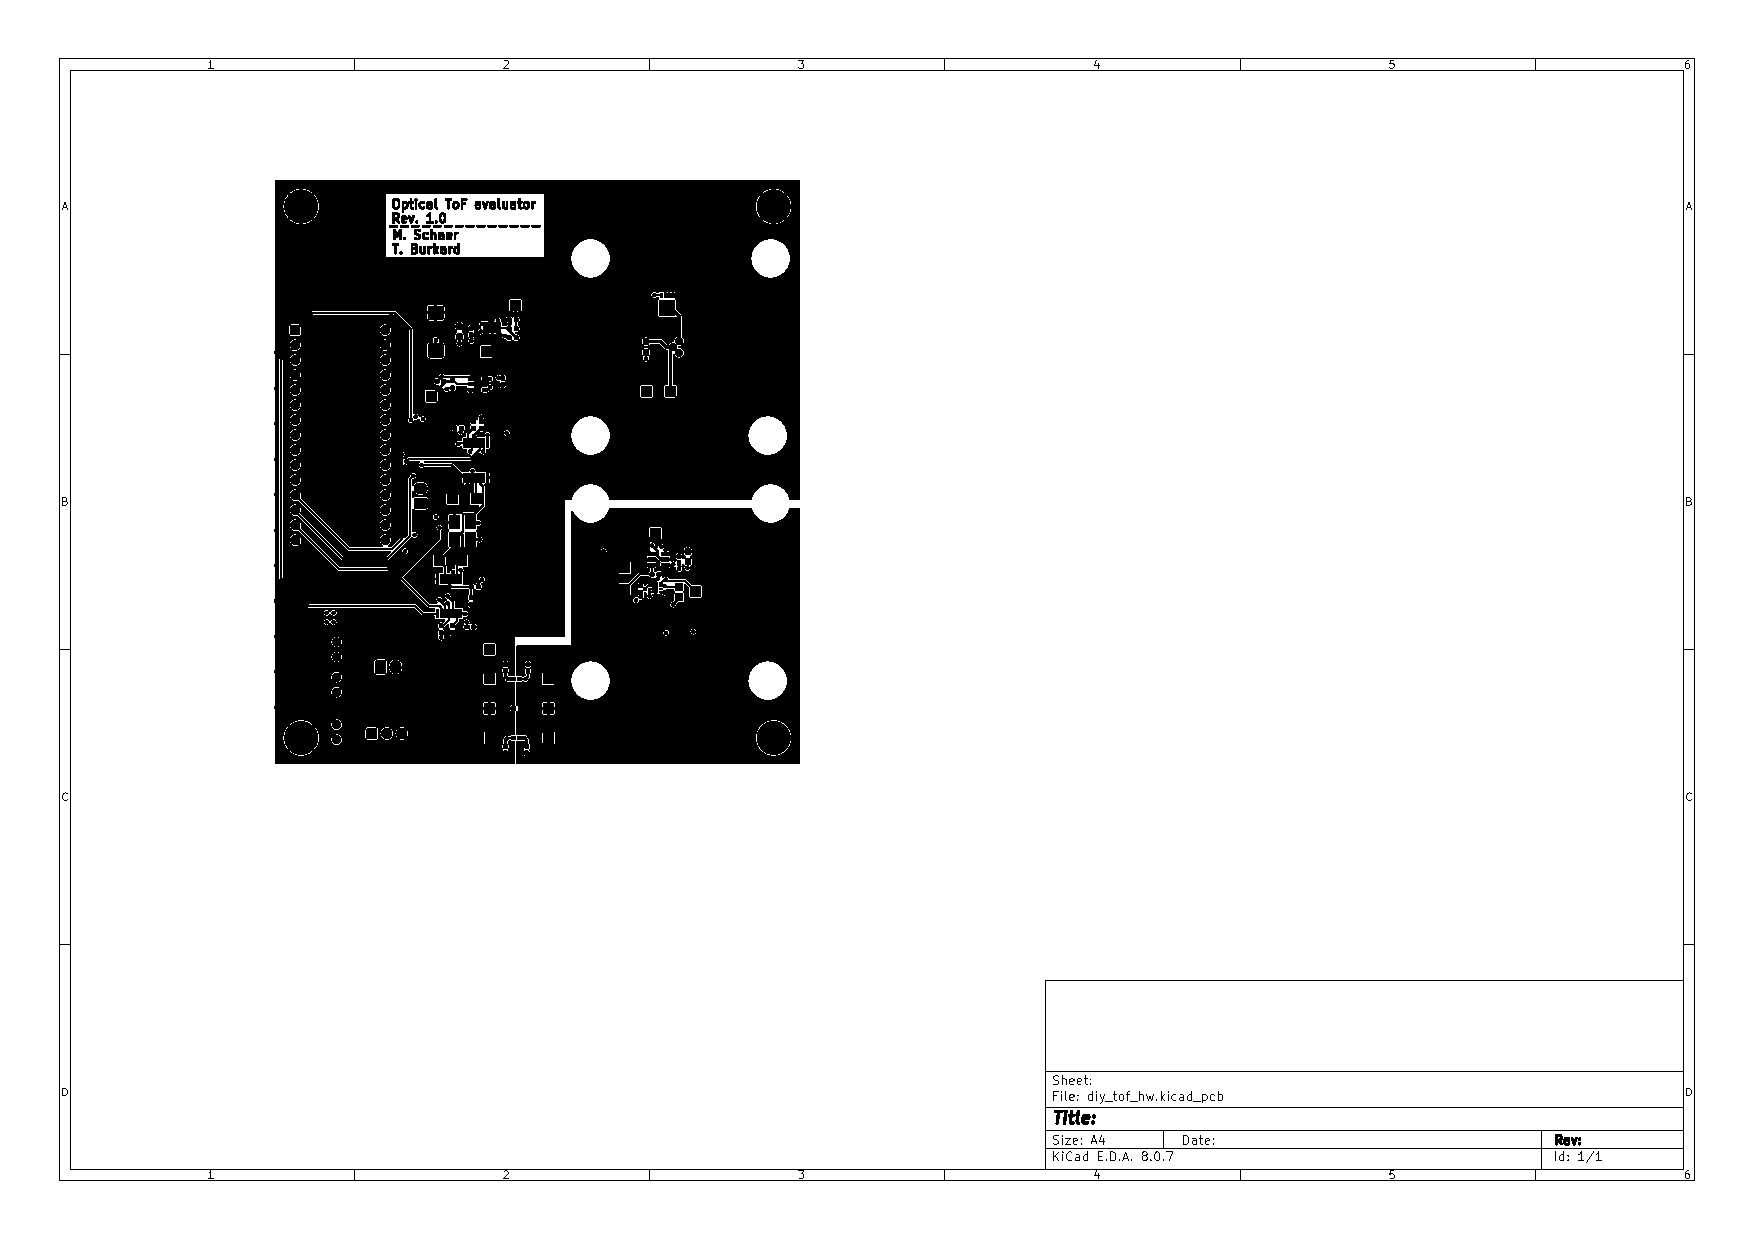
\includegraphics[trim=130 220 450 80, clip, width=0.6\textwidth]{attachments/pcb_F_Cu.pdf}
    \caption{PCB Layout Top}\label{fig:pcb_f_cu}
\end{figure}

\begin{figure}[H]
    \centering
    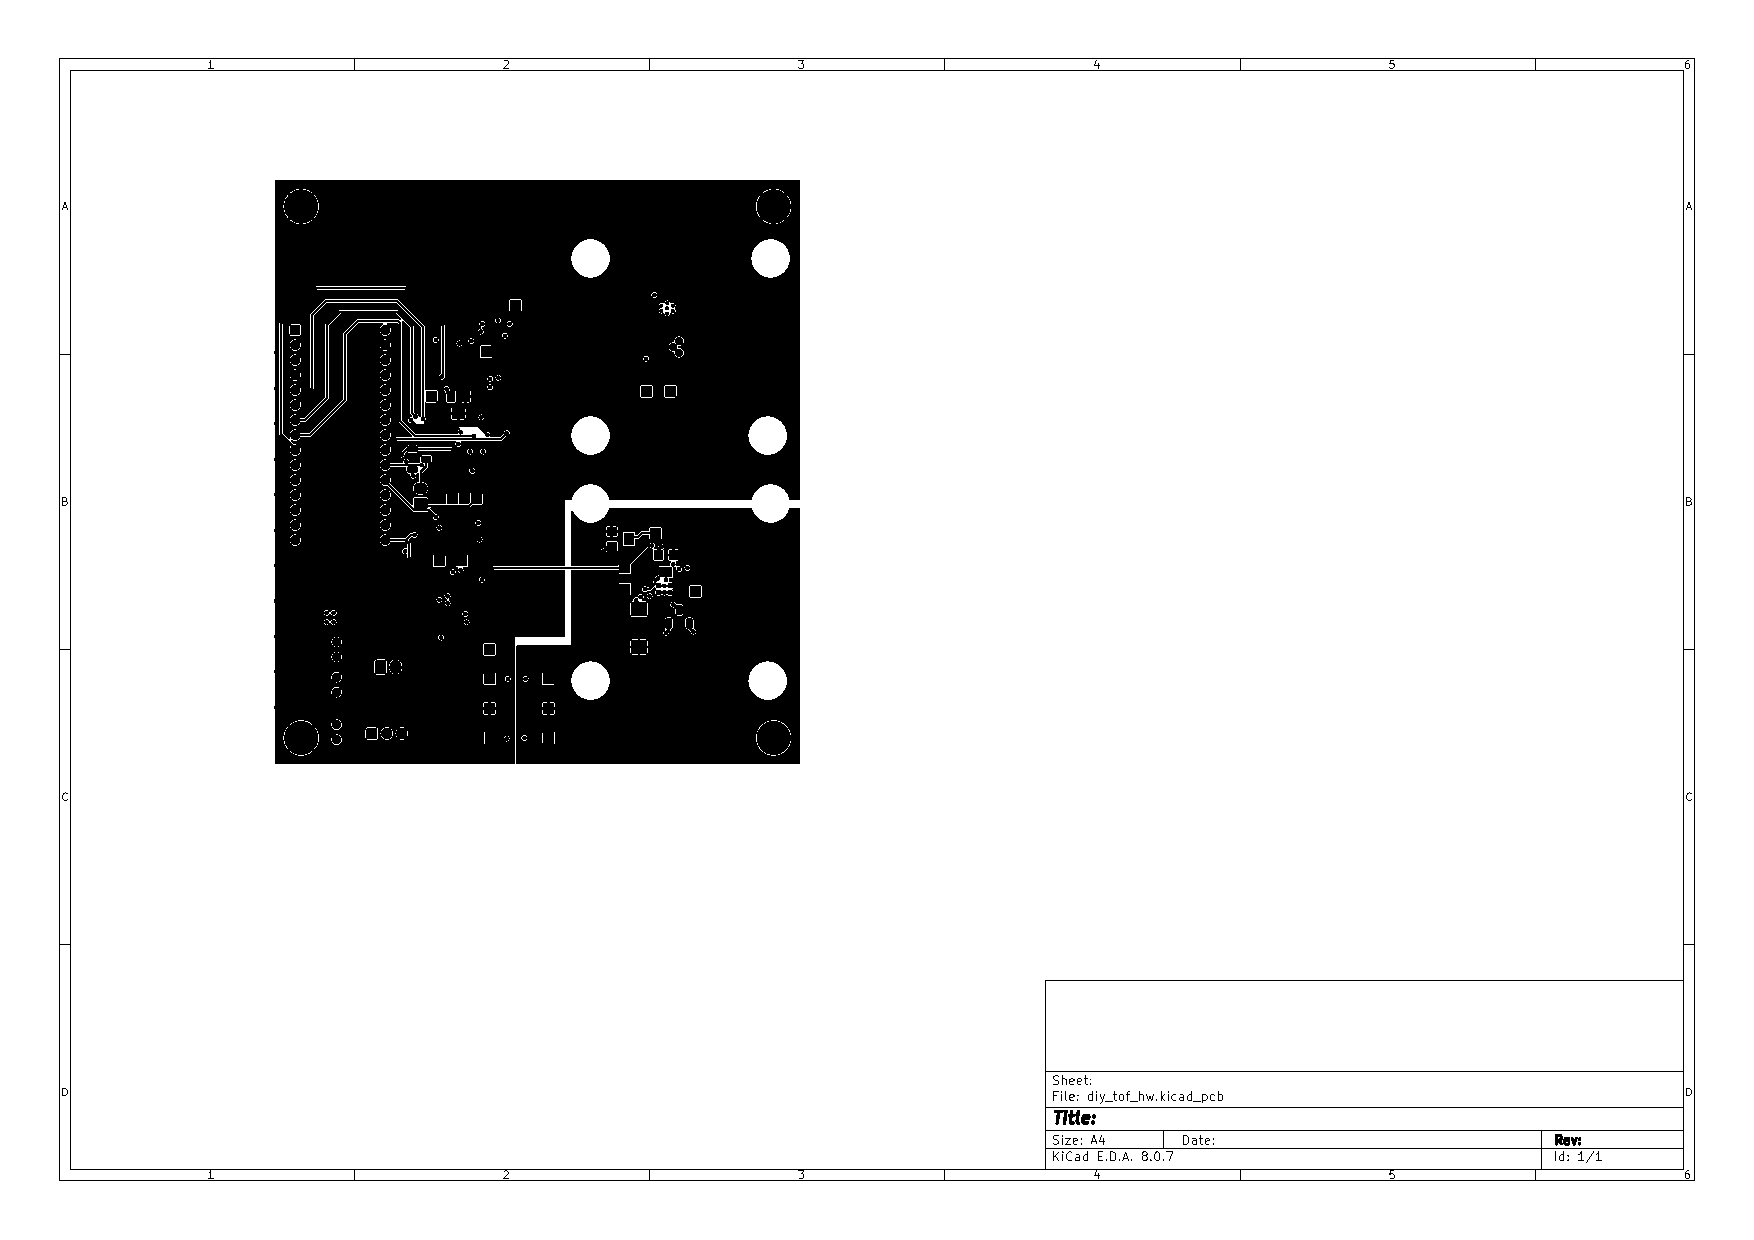
\includegraphics[trim=130 220 450 80, clip, width=0.6\textwidth]{attachments/pcb_B_Cu.pdf}
    \caption{PCB Layout Bottom}\label{fig:pcb_b_cu}
\end{figure}

\begin{figure}[H]
    \centering
    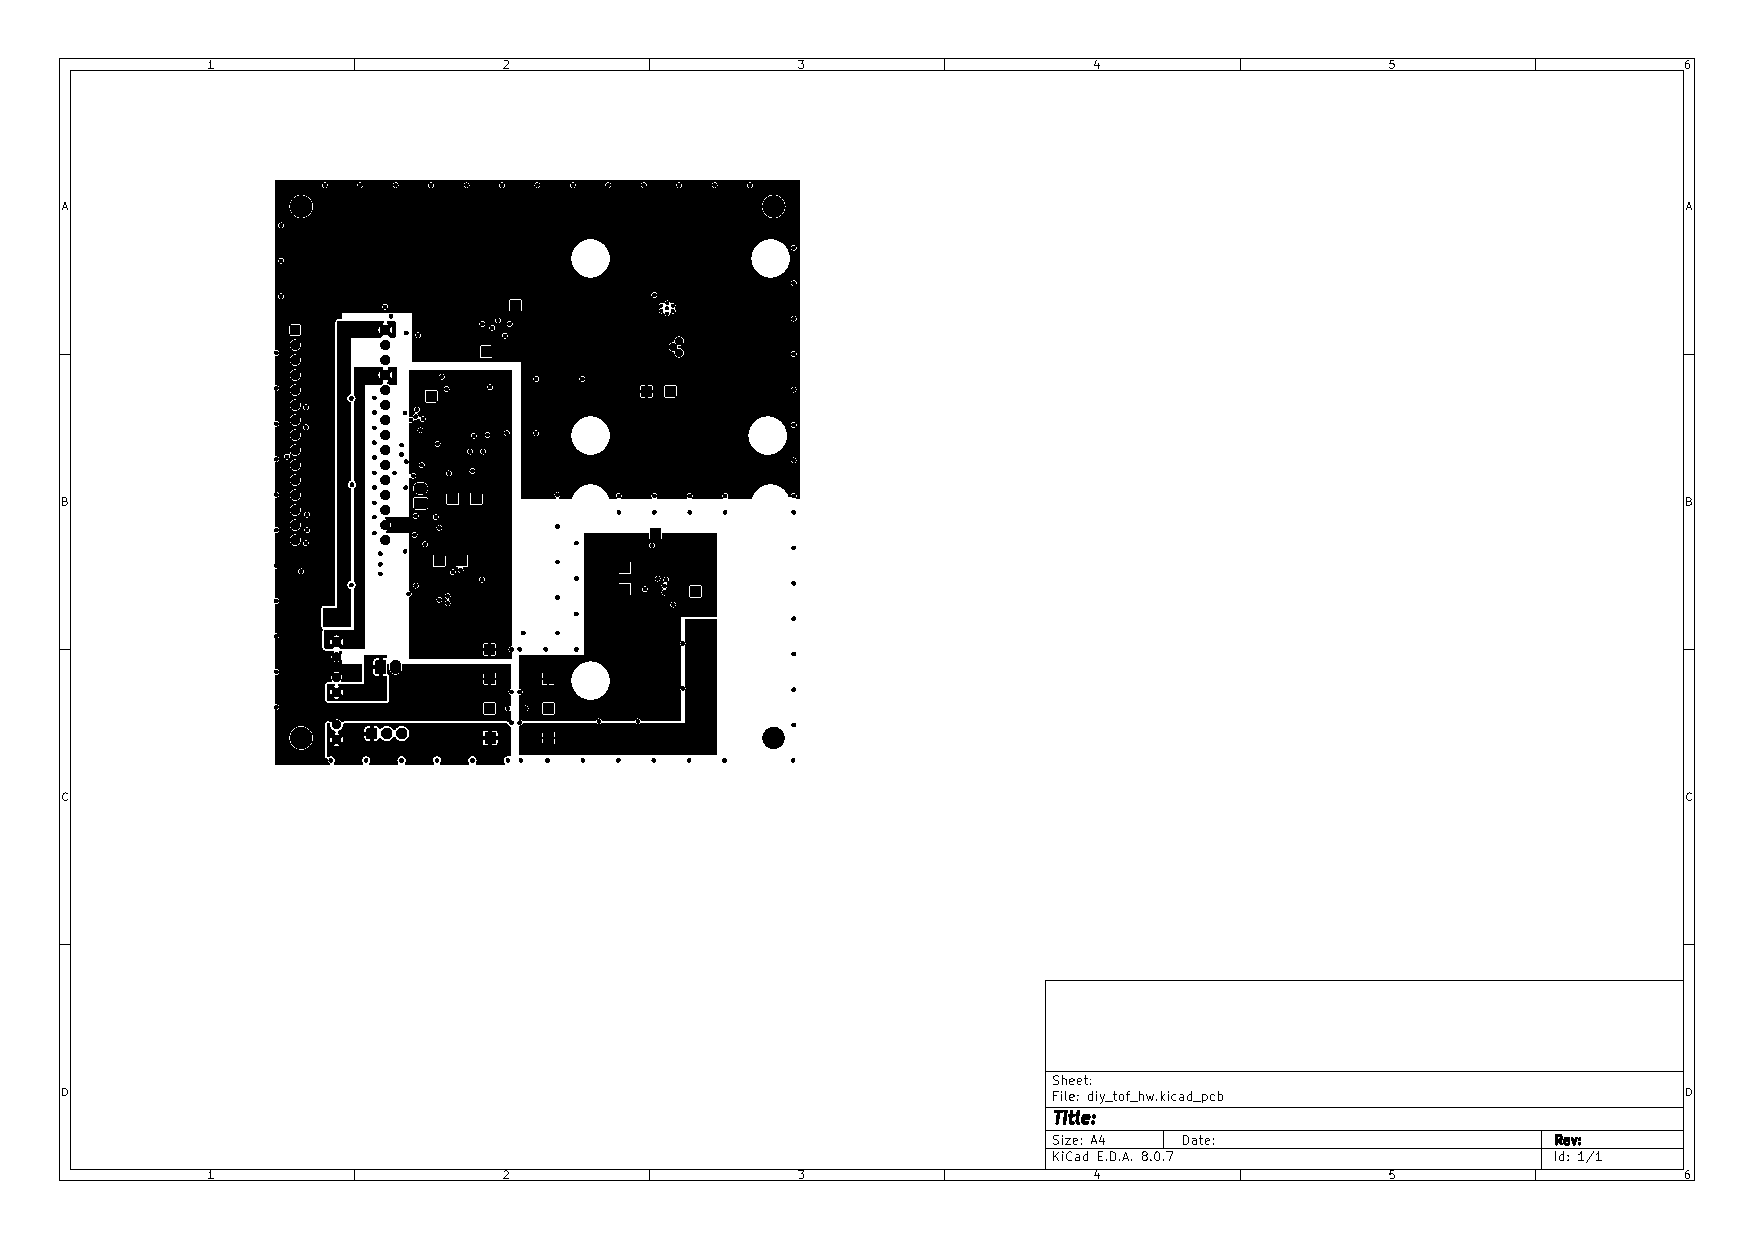
\includegraphics[trim=130 220 450 80, clip, width=0.6\textwidth]{attachments/pcb_In1_Cu.pdf}
    \caption{PCB Layout Innen 1}\label{fig:pcb_in1_cu}
\end{figure}

\begin{figure}[H]
    \centering
    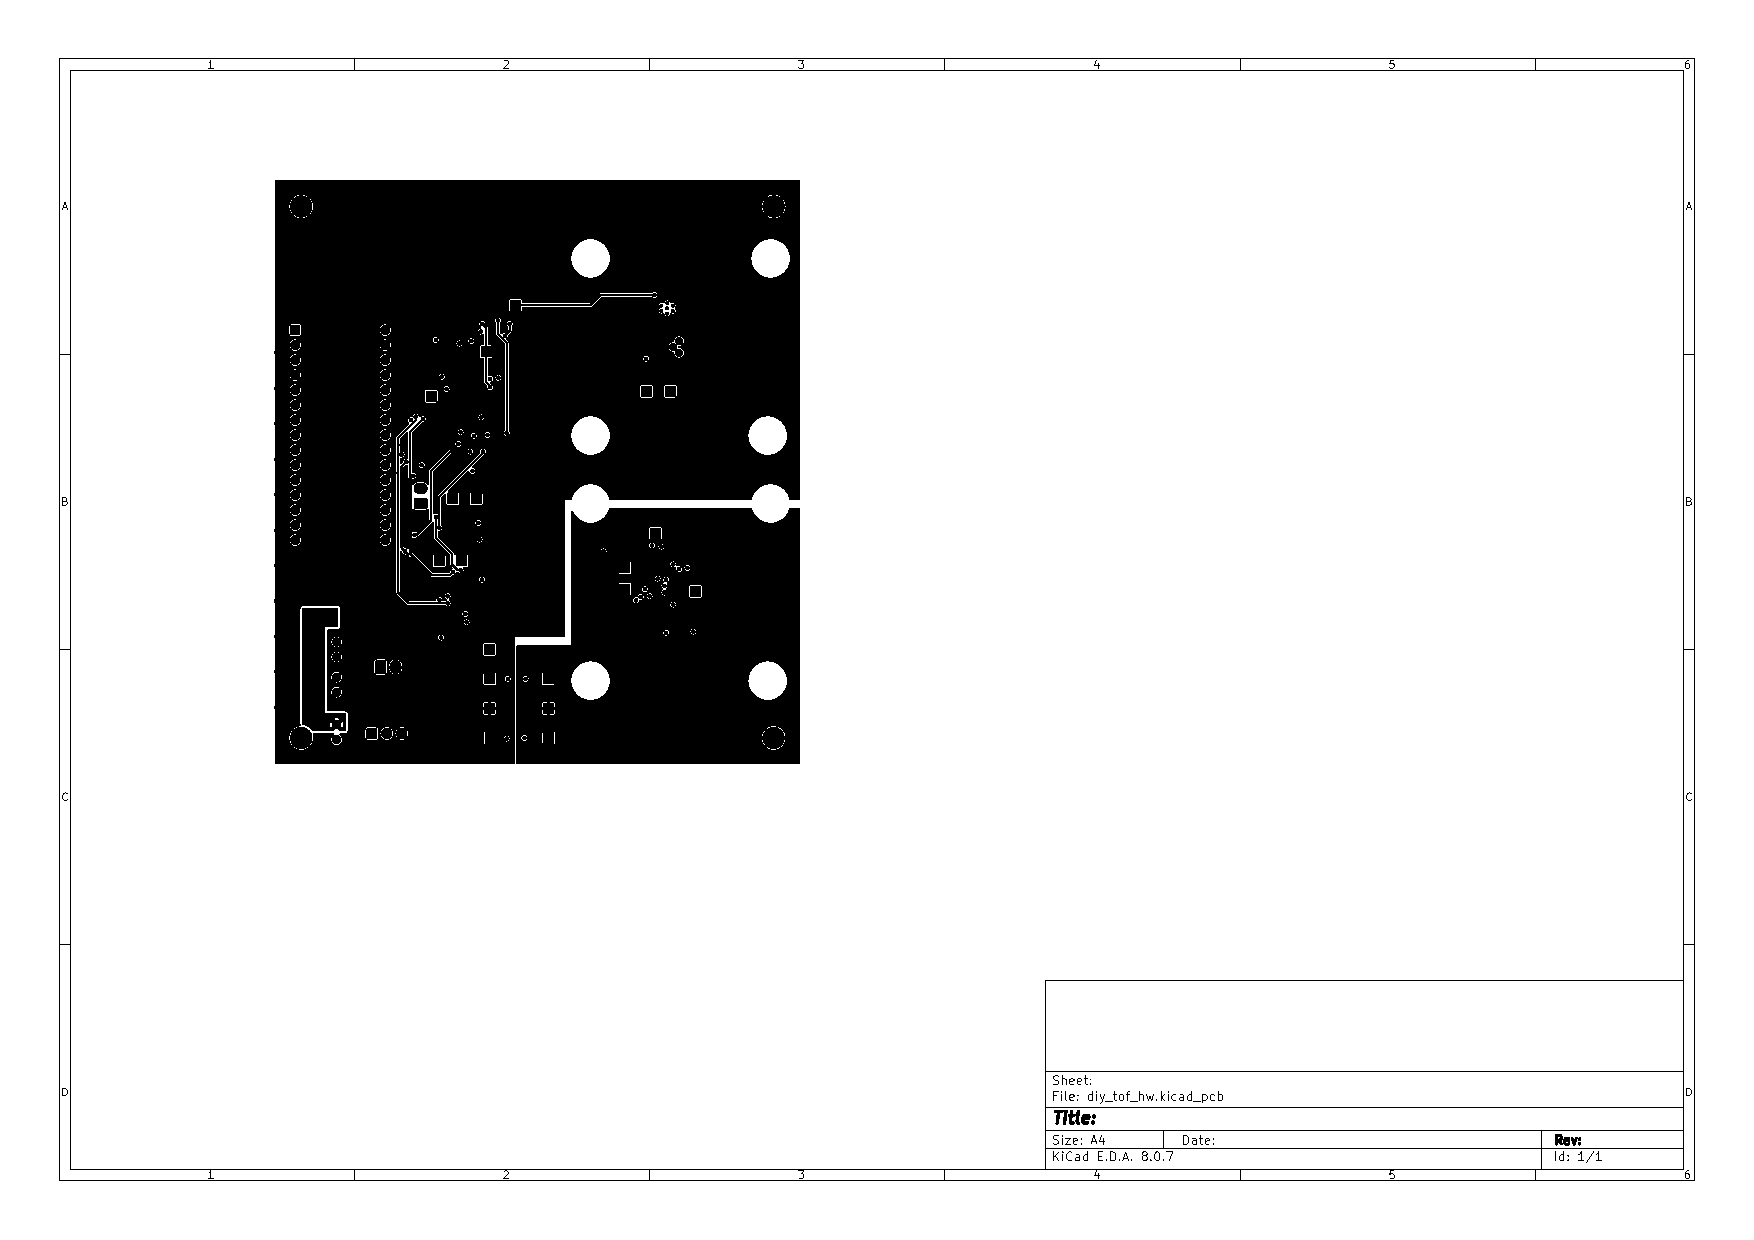
\includegraphics[trim=130 220 450 80, clip, width=0.6\textwidth]{attachments/pcb_In2_Cu.pdf}
    \caption{PCB Layout Innen 2}\label{fig:pcb_in2_cu}
\end{figure}

\subsubsection{Komponenten-Platzierung}

\begin{figure}[H]
    \centering
    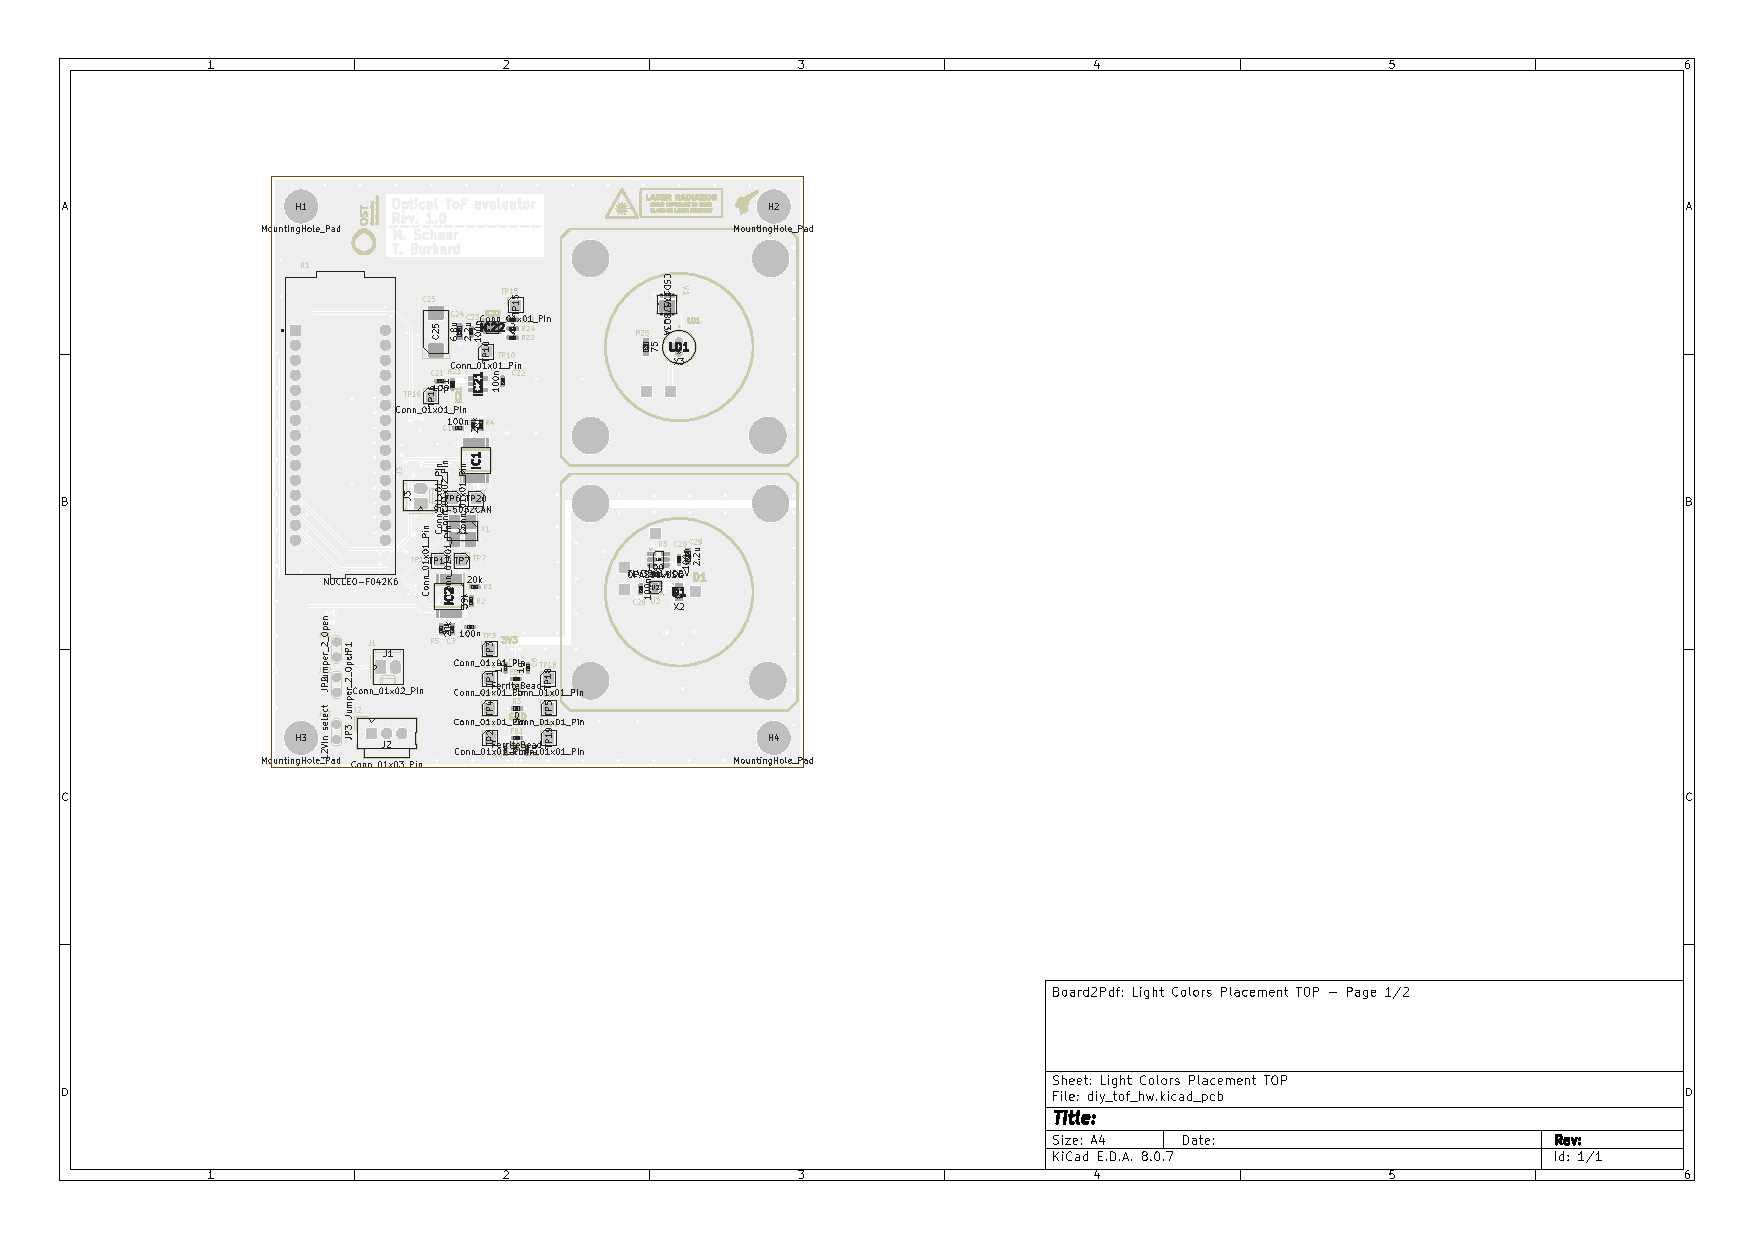
\includegraphics[page=1, trim=120 220 450 80, clip, width=0.6\textwidth]{attachments/pcb_placement.pdf}
    \caption{PCB Komponenten-Platzierung Top}\label{fig:pcb_placement_1}
\end{figure}

\begin{figure}[H]
    \centering
    \includegraphics[page=2, trim=450 220 120 80, clip, width=0.6\textwidth]{attachments/pcb_placement.pdf}
    \caption{PCB Komponenten-Platzierung Bottom}\label{fig:pcb_placement_2}
\end{figure}

\pagebreak

\subsection{3D View}

\begin{figure}[H]
    \centering
    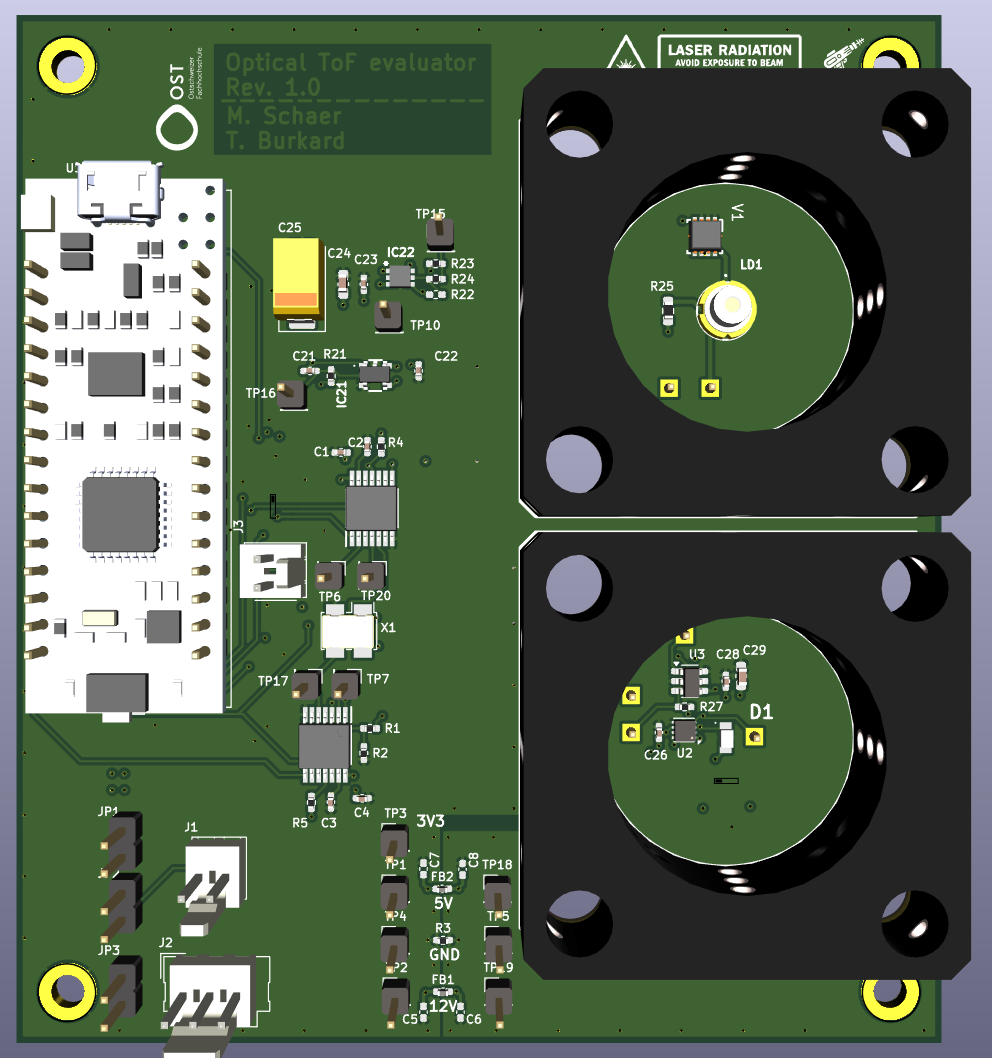
\includegraphics[width=0.6\textwidth]{graphics/3d_top.png}
    \caption{3D View Top}\label{fig:3d_top}
\end{figure}

\begin{figure}[H]
    \centering
    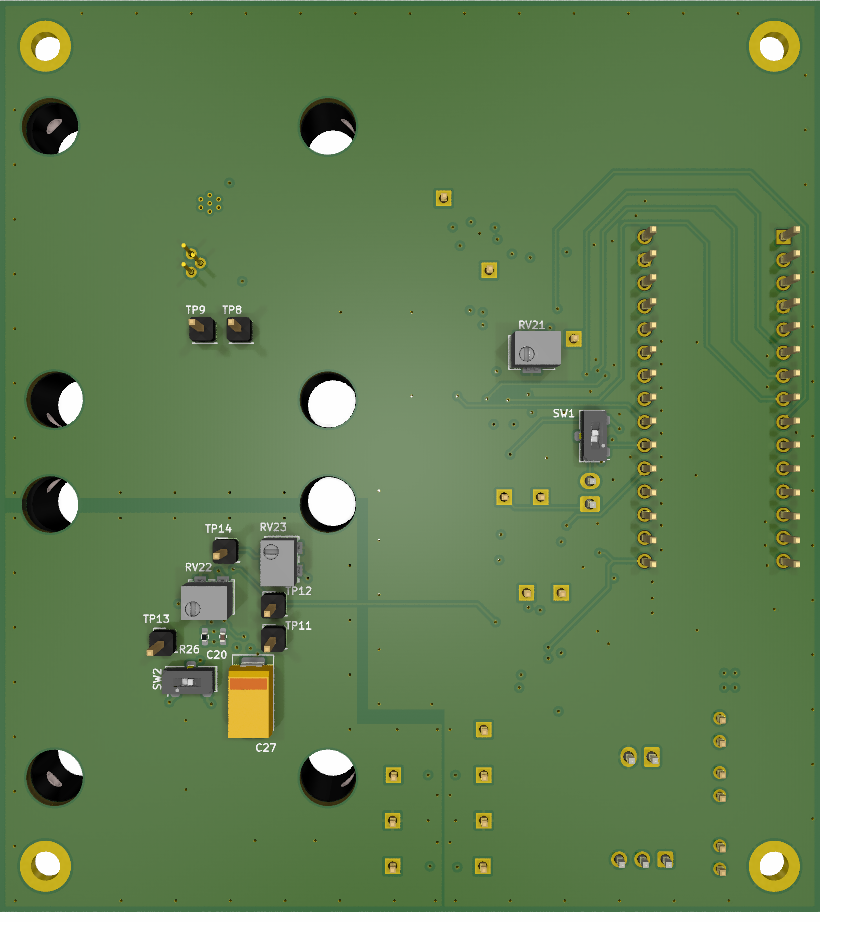
\includegraphics[width=0.6\textwidth]{graphics/3d_bottom.png}
    \caption{3D View Bottom}\label{fig:3d_bottom}
\end{figure}


\section[Resultate]{Resultate (8 min)}
\subsection{Elektrische Resultate}

\begin{frame}{Unterschiedliche Kabellängen}
    \begin{figure}
        \includesvg[width=0.8\textwidth]{../documentation/graphics/different_cable_lengths_with_dso_tdc.svg}
    \end{figure}
\end{frame}

\begin{frame}{Unterschiedliche Kabellängen: Resultate}
    \begin{table}
        \mytable
            {|l|l|l|l|}
            {\textbf{Länge} & \textbf{Mittelwert} & \textbf{Standardabweichung} & \textbf{$\Delta$ zu 0~m}}
            {\length & \mean & \stddev & \diff}
            {../documentation/tables/different_cable_lengths_with_dso_tdc.csv}
    \end{table}
\end{frame}

\begin{frame}{Unterschiedliche Kabellängen: Zurückgerechnet}
    \begin{table}
        \mytable
            {|l|l|}
            {\textbf{Länge} & \textbf{TDC zurückgerechnet mit 0.9~c}}
            {\length & \tdcgemtheoriemc}
            {../documentation/tables/different_cable_lengths_with_dso_theorie09_vs_tdc_m.csv}
    \end{table}
\end{frame}

\subsection{Optische Resultate}

\begin{frame}{Signalpfad Sender}
    \begin{figure}
        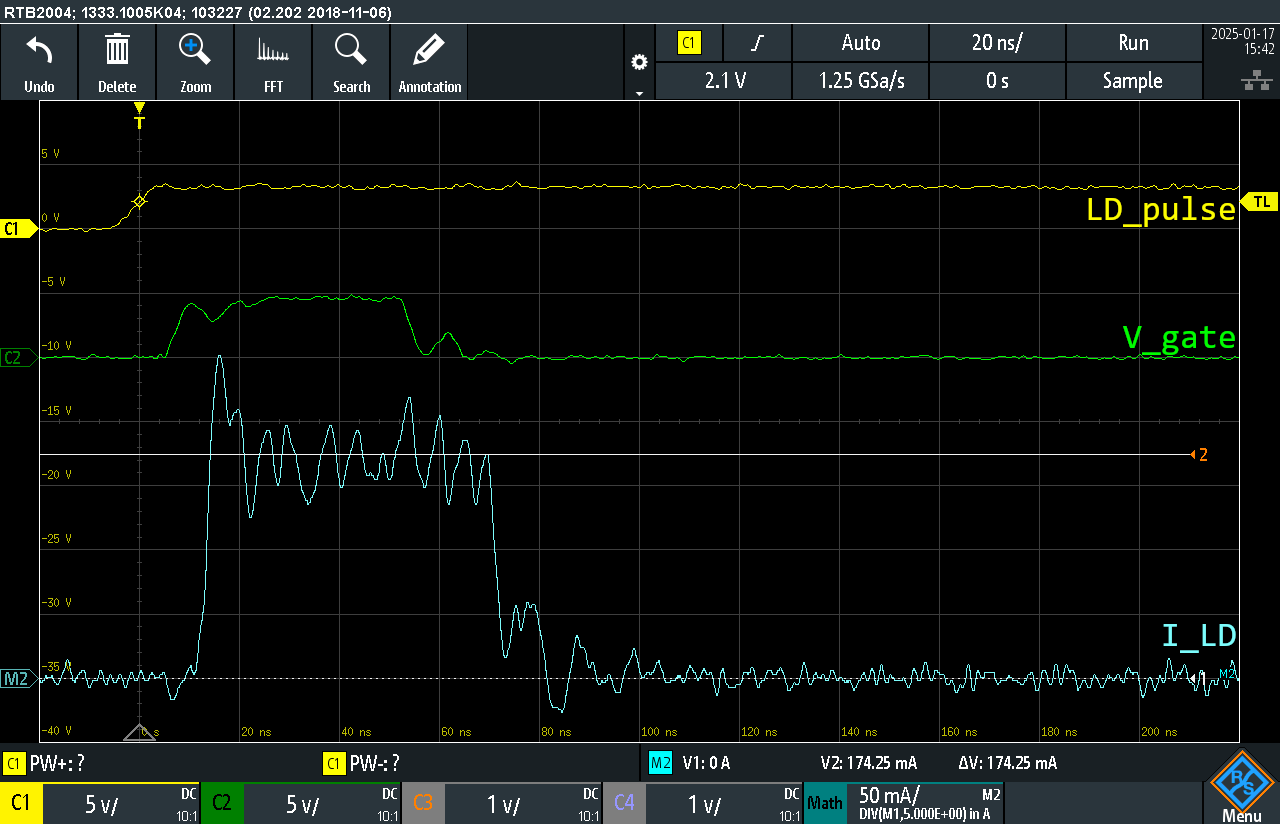
\includegraphics[width=0.7\textwidth]{../documentation/graphics/signalpfad_sender_ld_strom.png}
    \end{figure}
\end{frame}

\begin{frame}{ToF-Messungen via Spiegel}
    \begin{figure}
        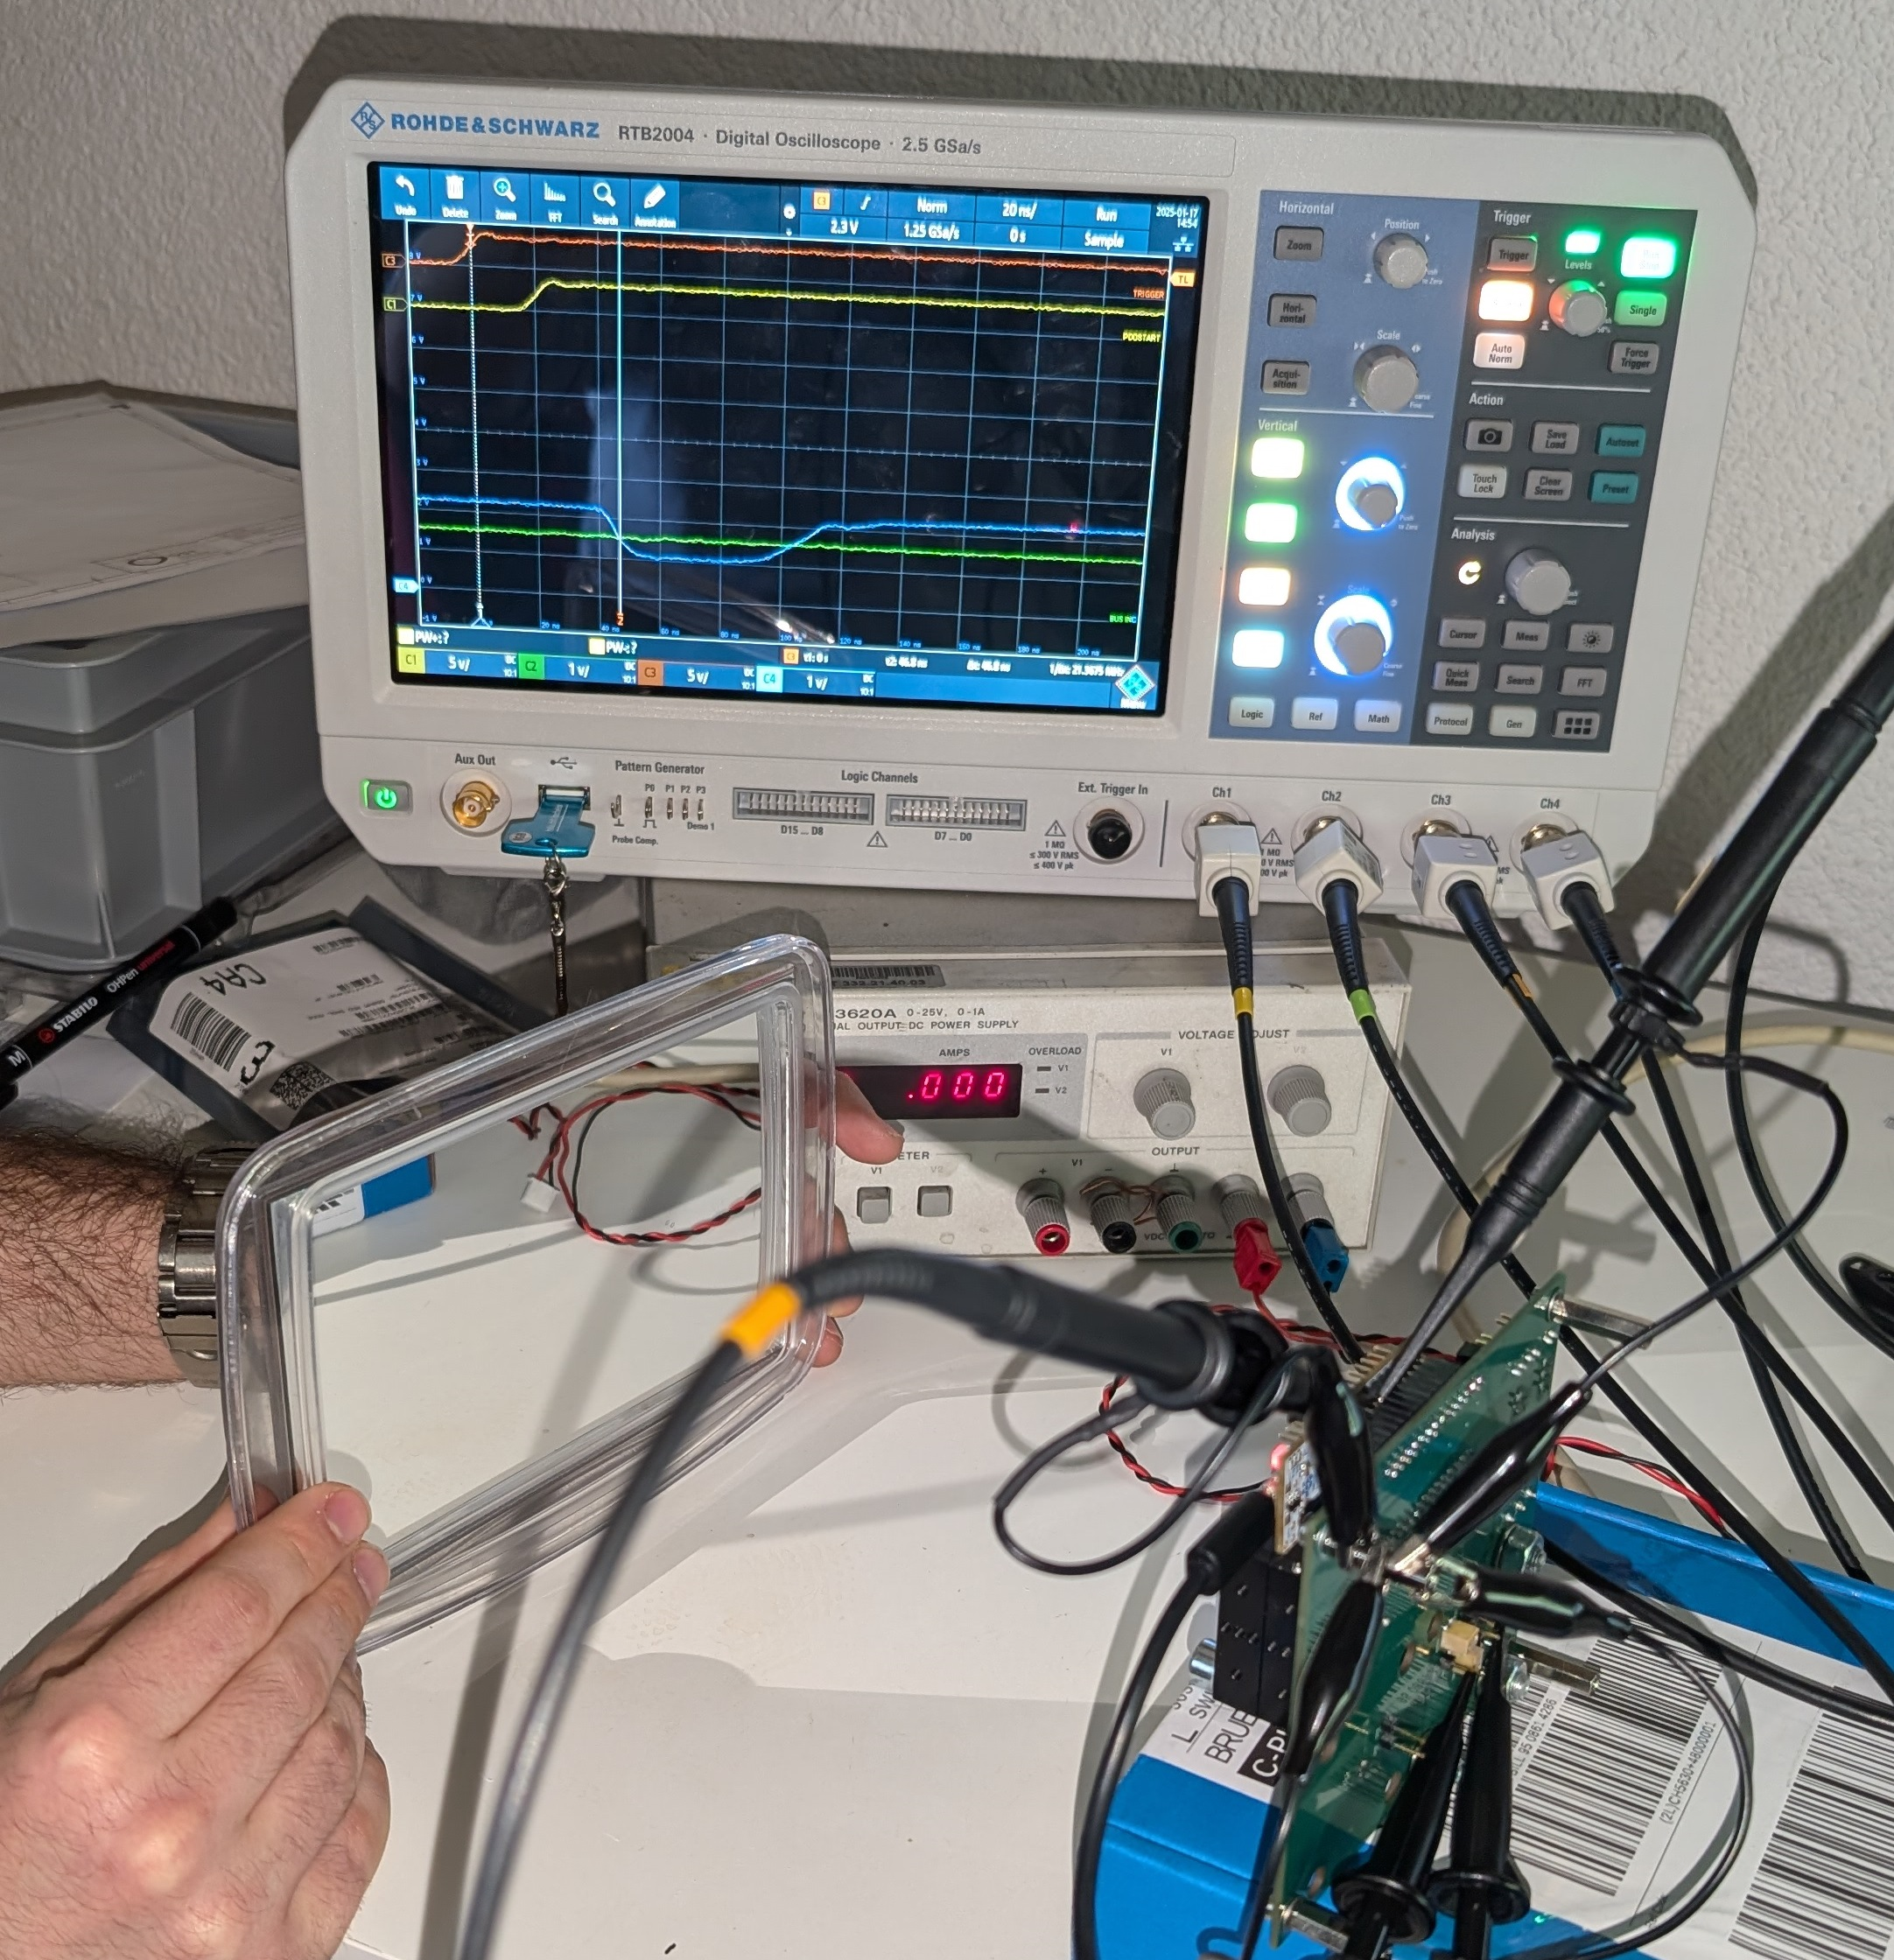
\includegraphics[width=0.45\textwidth]{../documentation/graphics/spiegel_setup.jpg}
    \end{figure}
\end{frame}

\begin{frame}{ToF-Messungen via Spiegel: DSO}
    \begin{figure}
        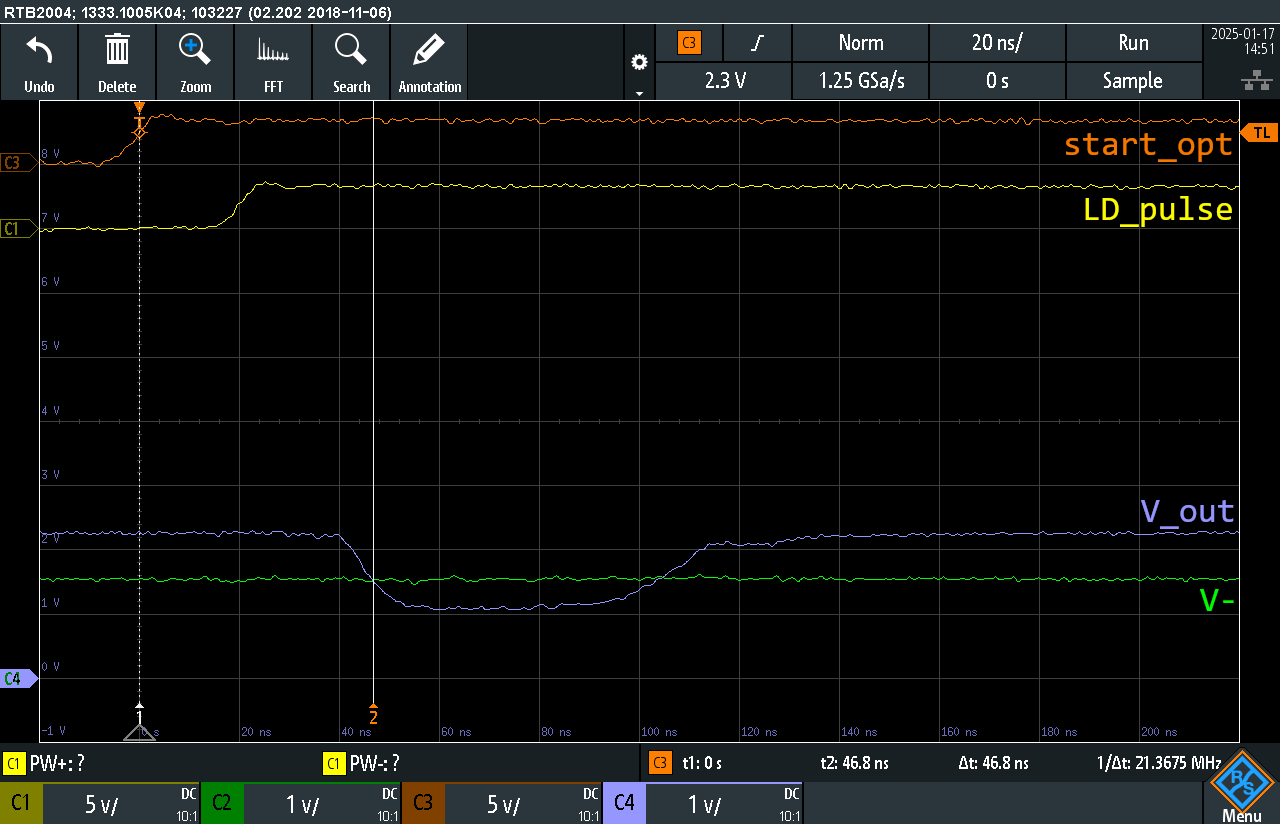
\includegraphics[width=0.7\textwidth]{../documentation/graphics/spiegel_12cm_dso_ok.png}
    \end{figure}
\end{frame}

\begin{frame}{ToF-Messungen via Spiegel: Resultate}
    \begin{figure}
        \includesvg[width=0.8\textwidth]{../documentation/graphics/spiegel_unterschiedliche_distanzen.svg}
    \end{figure}
\end{frame}

\begin{frame}{ToF-Messungen via Spiegel: Auswertung}
    \begin{table}
        \mytable
            {|l|l|l|}
            {\textbf{Distanz zum Spiegel} & \textbf{Mittelwert} & \textbf{Standardabweichung}}
            {\distance & \mean & \stddev}
            {../documentation/tables/spiegel_unterschiedliche_distanzen.csv}
    \end{table}

    \onslide<2->{
        \begin{equation*}
            \begin{split}
                \Delta ToF_{meas} &\approx 0.6~ns\\
                \Delta ToF_{calc} &= \frac{\Delta L}{c} = \frac{10~cm}{3 \cdot 10^8~m/s} = 0.33~ns
            \end{split}
        \end{equation*}
    }
\end{frame}

\begin{frame}{ToF-Messungen via Spiegel: Drift}
    \begin{figure}
        \includesvg[width=0.8\textwidth]{../documentation/graphics/spiegel_unterschiedliche_distanzen_linear.svg}
    \end{figure}
\end{frame}

\begin{frame}{ToF-Messungen via Spiegel: $>$30 cm}
    \begin{figure}
        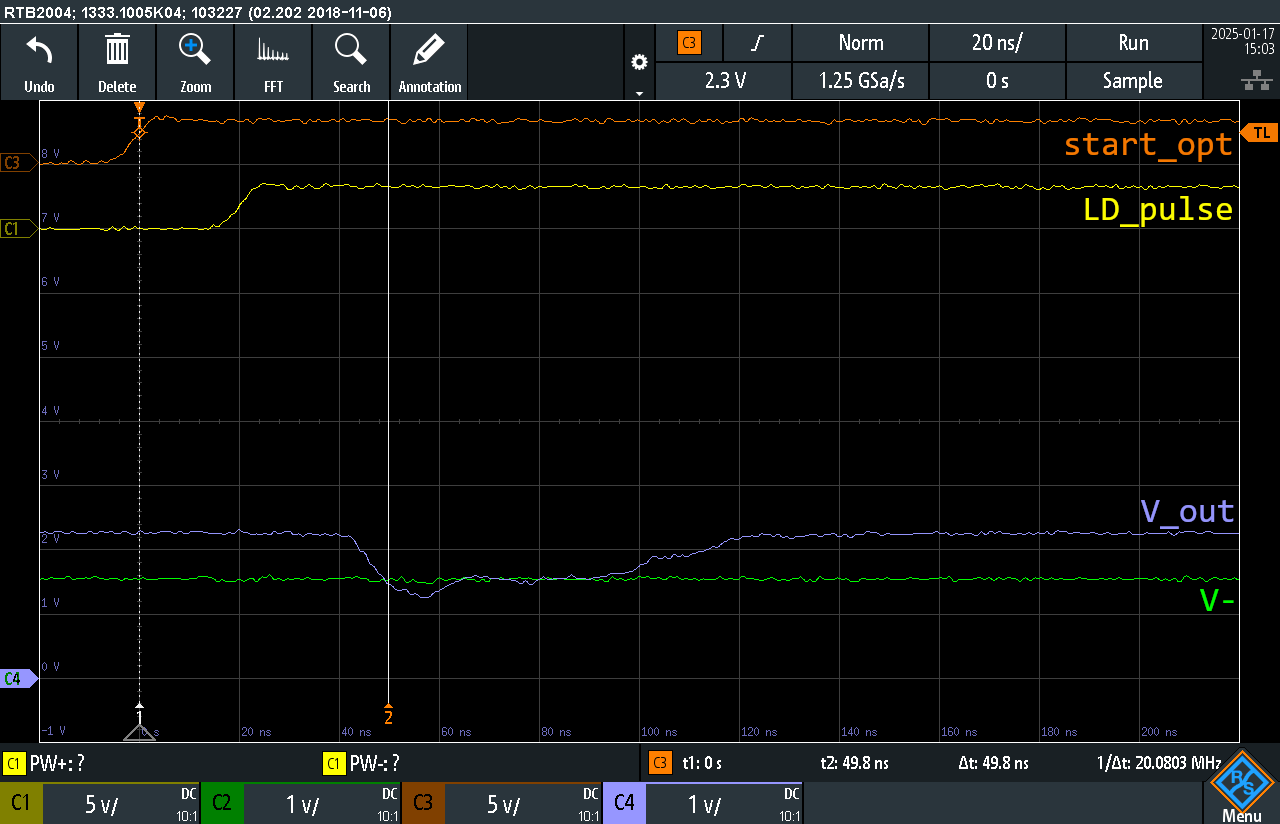
\includegraphics[width=0.7\textwidth]{../documentation/graphics/spiegel_30cm_dso_nok.png}
    \end{figure}
\end{frame}

\begin{frame}{ToF-Messungen via Wand}
    \begin{itemize}
        \item Leider keine brauchbaren Messresultate bis jetzt
    \end{itemize}
\end{frame}


\section[Fazit]{Fazit (3 min)}
In diesem Kapitel werden abschliessende Gedanken gesammelt. Es soll dazu dienen einen Ausblick zu geben für mögliche,
weiterführende Arbeiten. Es sollen auch einige Punkte aufzuzählen, die gut gelaufen sind, aber auch jene bei denen
Verbesserungspotential identifiziert wurde.

\subsection{Ausblick}\label{sec:ausblick}

Grundsätzlich kann bestätigt werden, dass sich ein \acrshort{tof}-System, so wie es sich die Studierenden vorstellen,
entwickeln und betreiben lässt. Nachfolgend werden ein paar mögliche Verbesserungen und weiterführende Messungen
aufgelistet.

\begin{enumerate}
    \item Die Optik besser aufeinander abstimmen. Dies würde es zum einen erlauben, über weitere Distanzen hinweg
          Messungen machen zu können. Des weiteren sollte es ebenfalls möglich sein, auch Targets mit nicht oder schwach
          reflektierenden Oberflächen-Beschaffenheiten zu detektieren.
    \item Für die Messungen mit dem Spiegel würde es Sinn machen mit einer Linse mit grösserer Brennweite (oder mit
          derselben Linse mit etwas weniger Distanz zum \acrshort{pcb}) auszuprobieren. Dies hätte den Vorteil, dass der
          Spiegel nicht ganz so genau ausgerichtet werden muss. Der Nachteil wäre etwas weniger Photostrom bei parallel
          einfallendem Licht.
    \item Bei der Ansteuerung der \acrshort{tdc}s gibt es Verbesserungspotential. So könnte beispielsweise mit einer
          schneller getakteten \acrshort{mcu} der Jitter bei \lstinline|START|- und \lstinline|STOP|-Signal minimiert
          werden, was zu Messresultaten mit noch weniger Streuung führen wird.
    \item Eine andere Möglichkeit um die Streuung zu senken, wäre es eine externe Clock-Quelle zu verwenden.
    \item Eventuell ist es möglich auf die künstlich eingefügte Verzögerungszeit von einem Taktzyklus zu verzichten.
          Dies wäre der Fall, falls im Messpfad bereits genug Verzögerung entsteht, um die minimale Messdauer von 12~ns
          zu überschreiten. Falls nicht, könnte die künstliche Verzögerung anstatt von der \acrshort{mcu} auch mittels
          separater Schaltung (mit möglichst tiefem Jitter) umgesetzt werden.
    \item Beim verwendeten Nucleo gibt es die Möglichkeit, die Anstiegszeit der \acrshort{gpio} zu konfigurieren. Mit
          schnellerer Anstiegszeit lassen sich evtl. die Messresultate verbessern.
    \item Optischer Empfangspfad: Es sollten Messungen mit unterschiedlichen Verstärkungen des \acrshort{tia}
          durchgeführt werden, um die Distanz mit Spiegel zu erhöhen und Messungen gegen die Wand oder andere Targets zu
          ermöglichen. Damit zusammenhängend sollte die Schaltschwelle des Komparators genauer ausgetestet und
          feinjustiert werden.
    \item Optischer Sendepfad: Es lohnt sich mit höherer Sendeleistung zu experimentieren. Aufgrund der 5~V Speisung
          der Laser-Diode sind wir mit dem $5~\Omega$ Vorwiderstand schon fast am Limit. In einer nächsten
          \acrshort{pcb}-Version würde es sich lohnen mit einem Schalter die Möglichkeit zur 12~V Speisung vorzusehen,
          analog dazu wie dies für die Photodiode bereits umgesetzt ist.
    \item Optische Messungen: Es lohnt sich zu analysieren, weshalb die Messresultate in zwei Clustern (ca. 2~ns
          auseinander liegend) verteilt sind.
    \item Für weitere Messungen mit einem Spiegel lohnt es sich einen präzisen, mechanischen Versuchsaufbau zu
          konstruieren. Bei diesem könnte der Spiegel besser fixiert und eingestellt werden. Von Hand ist es schwierig
          reproduzierbare Ergebnisse zu erzielen.
\end{enumerate}

Abschliessend kann gesagt werden, dass es durchaus möglich ist, mit einem TDC7200 eine \acrshort{tof}-Messung zu machen,
bei welcher die zeitliche Auflösung des Mess-\acrshort{ic}s selber die limitierende Grösse ist.

\subsection{Lessons Learned}

Wie die Messresultate und auch der Ausblick bereits vermuten lassen, hätte primär beim Auslegen der Optoelektronik etwas
mehr Zeit investiert werden können. Die initialen, überschlags-mässigen Schätzungen und Rechnungen bezüglich der gewünschten
Limitierungen des Systems hätten kritischer hinterfragt werden sollen. Initial war es das Ziel der Studenten, Messungen
auf Distanzen von bis zu 10~m mit einer Auflösung von etwa 10~cm zu machen. Herausgestellt hat sich am Ende jedoch, dass
nicht die zeitliche Auflösung, sondern vielmehr die Distanz, resp. die Stärke des Messsignals problematisch ist.

Mit der Fabrikation des \acrshort{tof}-Demonstrators ist das Studenten-Team zufrieden. Beim erneuten Einsatz so kleiner
SMD-Komponenten, wie beispielsweise beim \acrshort{tia} lohnt es sich jedoch darüber zu sinnieren, ob nicht eine
maschinelle Bestückung der händischen Bestückung vorzuziehen ist. Durch die manuelle Bestückung wurde wohl keine Zeit
eingespart, da diese auch einige Stunden über mehrere Abende verteilt in Anspruch nahm.

\subsection{Danksagung}

Wir möchten uns an dieser Stelle herzlich bei den beiden Dozenten Prof. Guido Keel und Michael Lehmann bedanken. Während
der Laufzeit des Projekts sind sie uns jederzeit mit Rat und Tat zur Seite gestanden und haben das Projekt mit grossem
Interesse verfolgt. Auch für das optische Leihmaterial bedanken wir uns. Dieses hat uns ermöglicht, bei der optischen
Messung einen Teilerfolg erzielen zu können.

Weiter bedanken wir uns bei Robin Burkard, der für uns ein Layout-Review durchgeführt hat. Dank seinen wertvollen Tipps
konnte das \acrshort{pcb} so störfrei wie möglich in Betrieb genommen werden.


\section[Demonstration]{Demonstration (5 min)}
\input{demonstration.tex}

%%%%%%%%%%%%%%%%%%%%%% CONTENT END %%%%%%%%%%%%%%%%%%%%%%

\miniframesoff

\questions{}

%\begin{frame}[allowframebreaks]{Quellen}
    \nocite{*} % add all sources to bibliography not just the cited ones
    \bibliographystyle{unsrtnat}
    {\scriptsize \bibliography{./references.bib}}
\end{frame}


\end{document}
